\documentclass[20pt]{extarticle}

\usepackage[paperwidth=48in,paperheight=36in,margin=0.55in]{geometry}
\usepackage[T1]{fontenc}
\usepackage{lmodern}
\usepackage{graphicx}
\usepackage{xcolor}
\usepackage{amsmath}
\usepackage{enumitem}
\usepackage{parskip}
\usepackage{ragged2e}
\usepackage{array}

\pagestyle{empty}
\setlength{\parindent}{0pt}
\setlength{\parskip}{0.18em}
\setlength{\tabcolsep}{6pt}
\linespread{1.05}

\definecolor{myblue}{RGB}{20,72,140}
\definecolor{mylight}{RGB}{245,247,250}
\definecolor{mydark}{RGB}{30,30,30}

% -------------------------------------------------
% Box styles
% -------------------------------------------------
\newcommand{\posterboxone}[2]{%
  \noindent
  \fcolorbox{myblue}{mylight}{%
    \begin{minipage}[t]{0.985\linewidth}
      \vspace*{0.22cm}
      {\color{white}\fcolorbox{myblue}{myblue}{%
        \parbox[c][1.08cm][c]{0.975\linewidth}{\hspace{0.5cm}\bfseries\Large #1}
      }}\\[0.32cm]
      \color{mydark}
      #2
      \vspace*{0.28cm}
    \end{minipage}
  }
  \vspace*{0.65cm}
}

\newcommand{\posterboxtwo}[2]{%
  \noindent
  \fcolorbox{myblue}{mylight}{%
    \begin{minipage}[t]{0.985\linewidth}
      \vspace*{0.22cm}
      {\color{white}\fcolorbox{myblue}{myblue}{%
        \parbox[c][1.08cm][c]{0.975\linewidth}{\hspace{0.5cm}\bfseries\Large #1}
      }}\\[0.32cm]
      \color{mydark}
      #2
      \vspace*{0.28cm}
    \end{minipage}
  }
  \vspace*{1.10cm}
}

\newcommand{\posterboxthree}[2]{%
  \noindent
  \fcolorbox{myblue}{mylight}{%
    \begin{minipage}[t]{0.985\linewidth}
      \vspace*{0.22cm}
      {\color{white}\fcolorbox{myblue}{myblue}{%
        \parbox[c][1.08cm][c]{0.975\linewidth}{\hspace{0.5cm}\bfseries\Large #1}
      }}\\[0.32cm]
      \color{mydark}
      #2
      \vspace*{0.28cm}
    \end{minipage}
  }
  \vspace*{1.45cm}
}

\begin{document}
\color{mydark}

% =========================================================
% HEADER
% =========================================================
\noindent
\fcolorbox{myblue}{myblue}{%
    \begin{minipage}[c][3.2cm][c]{0.988\linewidth}
        \centering
        {\color{white}\bfseries\fontsize{29}{32}\selectfont
            Racketlon Match Prediction with Dynamic Ratings,\\
            Boosted Trees, and Geometric Confidence Analysis
        }\\[0.10cm]
        {\color{white}\fontsize{17}{19}\selectfont
        Zain Magdon-Ismail \quad | \quad Rensselaer Polytechnic Institute \quad | \quad RCOS
        }
    \end{minipage}
}

\vspace*{0.40cm}

% =========================================================
% THREE-COLUMN BODY
% =========================================================
\noindent
\begin{minipage}[t][31.8in][t]{\textwidth}

    % ---------------- LEFT COLUMN ----------------
    \begin{minipage}[t]{0.29\textwidth}
        \vspace*{0.65cm}

        \posterboxone{Motivation and Problem}{
            \justifying
            Racketlon combines four sports---table tennis (TT), badminton (BD), squash (SQ), and tennis (TN)---into one total-points match.

            This project built a full pipeline to:
            \begin{itemize}[leftmargin=1.15em,itemsep=0.06em,topsep=0.06em]
                \item scrape historical match data,
                \item clean and normalize records,
                \item build leakage-safe pre-match features,
                \item predict sport scores and match winner,
                \item study confidence using KD-tree geometry.
            \end{itemize}
        }

        \posterboxone{Pipeline Overview}{
            \vspace*{0.18cm}
            \begin{center}
                % IMAGE: poster_images/pipeline.png
                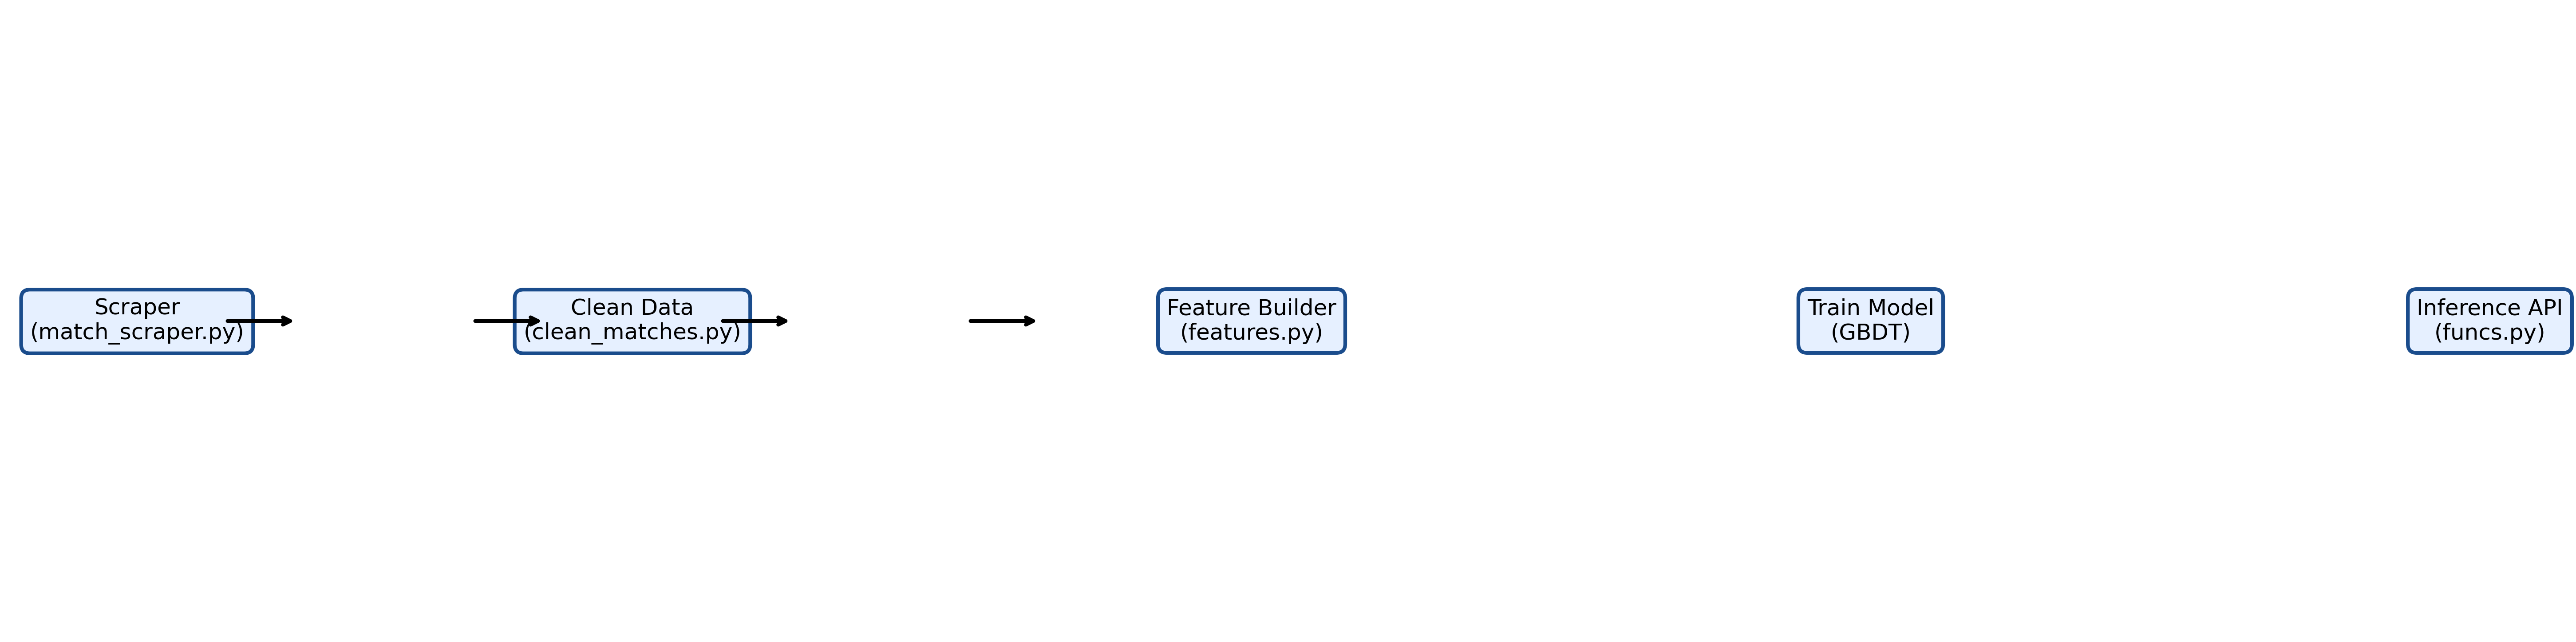
\includegraphics[width=0.42\linewidth]{poster_images/pipeline.png}
            \end{center}
            \vspace*{0.16cm}

            \textbf{Stages}
            \begin{enumerate}[leftmargin=1.25em,itemsep=0.05em,topsep=0.05em]
                \item scrape tournament data
                \item clean invalid matches
                \item build chronological features
                \item train sport-level regressors
                \item combine sport predictions
                \item analyze confidence
            \end{enumerate}
        }

        \posterboxone{Data and Cleaning}{
            \justifying
            Historical results were scraped from Tournament Software / FIR pages using a hybrid parser for both new and legacy formats.

            Removed rows:
            \begin{itemize}[leftmargin=1.15em,itemsep=0.05em,topsep=0.05em]
                \item doubles, mixed, team, and league events
                \item incomplete matches
                \item invalid or missing dates
                \item rows missing required scores
            \end{itemize}

            Players were normalized into canonical lowercase names.
        }

        \posterboxone{Feature Engineering}{
            \justifying
            Features were built chronologically, so each row only uses information available before the match.

            Main feature groups:
            \begin{itemize}[leftmargin=1.15em,itemsep=0.05em,topsep=0.05em]
                \item sport-specific rating differences
                \item recent rolling form
                \item residual performance vs expectation
                \item long-term shrunk means
                \item head-to-head statistics
                \item inactivity and time multipliers
            \end{itemize}
        }

        \posterboxone{Dynamic Rating Model}{
            \justifying
            Expected score difference:
            \[
                \hat{d} = 21 \tanh\left(\frac{\alpha (R_{p1}-R_{p2})}{2}\right)
            \]

            with:
            \[
                \alpha_{TT}=0.060,\quad
                \alpha_{BD}=0.080,\quad
                \alpha_{SQ}=0.060,\quad
                \alpha_{TN}=0.040
            \]

            Learning rate:
            \[
                \eta(g)=\eta_{\min}+(\eta_{\max}-\eta_{\min})e^{-g/\tau}
            \]

            Time multiplier:
            \[
                t_{\mathrm{mult}} = 1 + c_s\left(1-e^{-d/\tau_s}\right)
            \]
        }

        % extra separation so the final image box reads as its own section
        \vspace*{0.35cm}

        \posterboxthree{Winner Confusion Matrix}{
            \vspace*{0.22cm}
            \begin{center}
                % IMAGE: poster_images/winner_confusion_matrix.png
                
\includegraphics[width=0.65\linewidth]{poster_images/winner_confusion_matrix.png}
            \end{center}
            \vspace*{0.20cm}
        }

    \end{minipage}
    \hspace{0.015\textwidth}
    % ---------------- MIDDLE COLUMN ----------------
    \begin{minipage}[t]{0.31\textwidth}
        \vspace*{0.65cm}

        \posterboxtwo{Final Predictive Model}{
            \justifying
            The final system is a stacked gradient-boosted decision tree regression model trained separately for each sport.

            For each sport:
            \begin{itemize}[leftmargin=1.15em,itemsep=0.05em,topsep=0.05em]
                \item base differential model
                \item residual correction model
                \item total-points model
            \end{itemize}

            Final sport differential:
            \[
                \hat{d} = b + 0.7r
            \]

            This gave the best balance of accuracy, stability, and deployability.
        }

        \posterboxtwo{Hyperparameters}{
            \textbf{Base differential model}
            \begin{itemize}[leftmargin=1.15em,itemsep=0.04em,topsep=0.04em]
                \item 900 iterations
                \item depth 5
                \item learning rate 0.03
                \item RMSE objective
                \item $L_2$ regularization = 6
            \end{itemize}

            \textbf{Residual differential model}
            \begin{itemize}[leftmargin=1.15em,itemsep=0.04em,topsep=0.04em]
                \item 700 iterations
                \item depth 5
                \item learning rate 0.03
                \item RMSE objective
                \item $L_2$ regularization = 6
            \end{itemize}

            \textbf{Total model}
            \begin{itemize}[leftmargin=1.15em,itemsep=0.04em,topsep=0.04em]
                \item 800 iterations
                \item depth 6
                \item learning rate 0.03
                \item MAE objective
                \item $L_2$ regularization = 6
            \end{itemize}
        }

        \posterboxtwo{Main Results Summary}{
            \justifying
            Final performance:
            \begin{itemize}[leftmargin=1.15em,itemsep=0.06em,topsep=0.06em]
                \item Match total-difference MAE: about 13.8
                \item Winner accuracy: about 73\%
            \end{itemize}

            The final model predicts:
            \begin{itemize}[leftmargin=1.15em,itemsep=0.05em,topsep=0.05em]
                \item sport-level score differences
                \item sport-level total points
                \item total match differential
                \item final winner
            \end{itemize}
        }

        \posterboxtwo{KD-Tree Confidence Insight}{
            \justifying
            To connect the project to computational geometry, KD-trees were used to analyze local neighborhood structure in matchup feature space.

            Key idea:
            \begin{itemize}[leftmargin=1.15em,itemsep=0.05em,topsep=0.05em]
                \item dense historical neighborhoods $\rightarrow$ higher confidence
                \item sparse historical neighborhoods $\rightarrow$ lower confidence
            \end{itemize}

            This intuition works naturally for local models such as KNN, but was less effective for the final boosted-tree predictor.
        }

        \posterboxtwo{Practical Output}{
            \justifying
            The saved package supports:
            \begin{itemize}[leftmargin=1.15em,itemsep=0.05em,topsep=0.05em]
                \item training on full historical data
                \item loading saved models
                \item predicting future matchups by player name
                \item returning sport-level and full-match outcomes
            \end{itemize}
        }

        \posterboxtwo{Conclusion}{
            \justifying
            \begin{itemize}[leftmargin=1.15em,itemsep=0.06em,topsep=0.06em]
                \item Dynamic ratings and structured pre-match features are strong predictors of Racketlon outcomes.
                \item The final boosted-tree model gave the best balance of accuracy, stability, and deployability.
                \item KD-tree neighborhood analysis provided a computational-geometry interpretation of confidence.
                \item The complete system works end-to-end: scraping, cleaning, features, training, packaging, and future-match inference.
            \end{itemize}
        }

        \vspace*{0.25cm}

        \posterboxthree{Actual Match}{
            \vspace*{0.22cm}
            \begin{center}
                % IMAGE: poster_images/actual_match_photo.png
                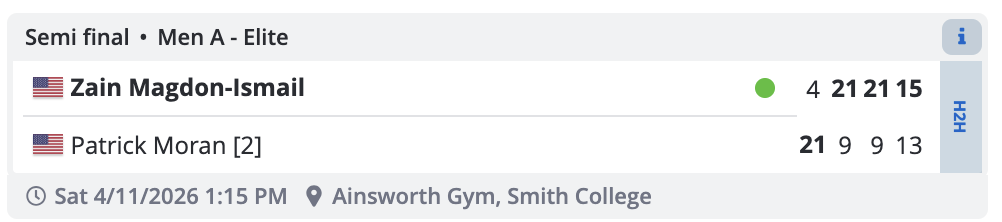
\includegraphics[width=0.70\linewidth]{poster_images/actual_match_photo.png}
            \end{center}
            \vspace*{0.20cm}
        }

    \end{minipage}
    \hspace{0.015\textwidth}
    % ---------------- RIGHT COLUMN ----------------
    \begin{minipage}[t]{0.35\textwidth}
        \vspace*{0.65cm}

        \posterboxthree{Match Total Difference: Actual vs Predicted}{
            \vspace*{0.22cm}
            \begin{center}
                % IMAGE: poster_images/match_total_diff_scatter.png
                
\includegraphics[width=0.50\linewidth]{poster_images/match_total_diff_scatter.png}
            \end{center}
            \vspace*{0.20cm}
        }

        \posterboxthree{KD-Tree Neighborhood Intuition}{
            \vspace*{0.22cm}
            \begin{center}
                % IMAGE: poster_images/kdtree_diagram.png
                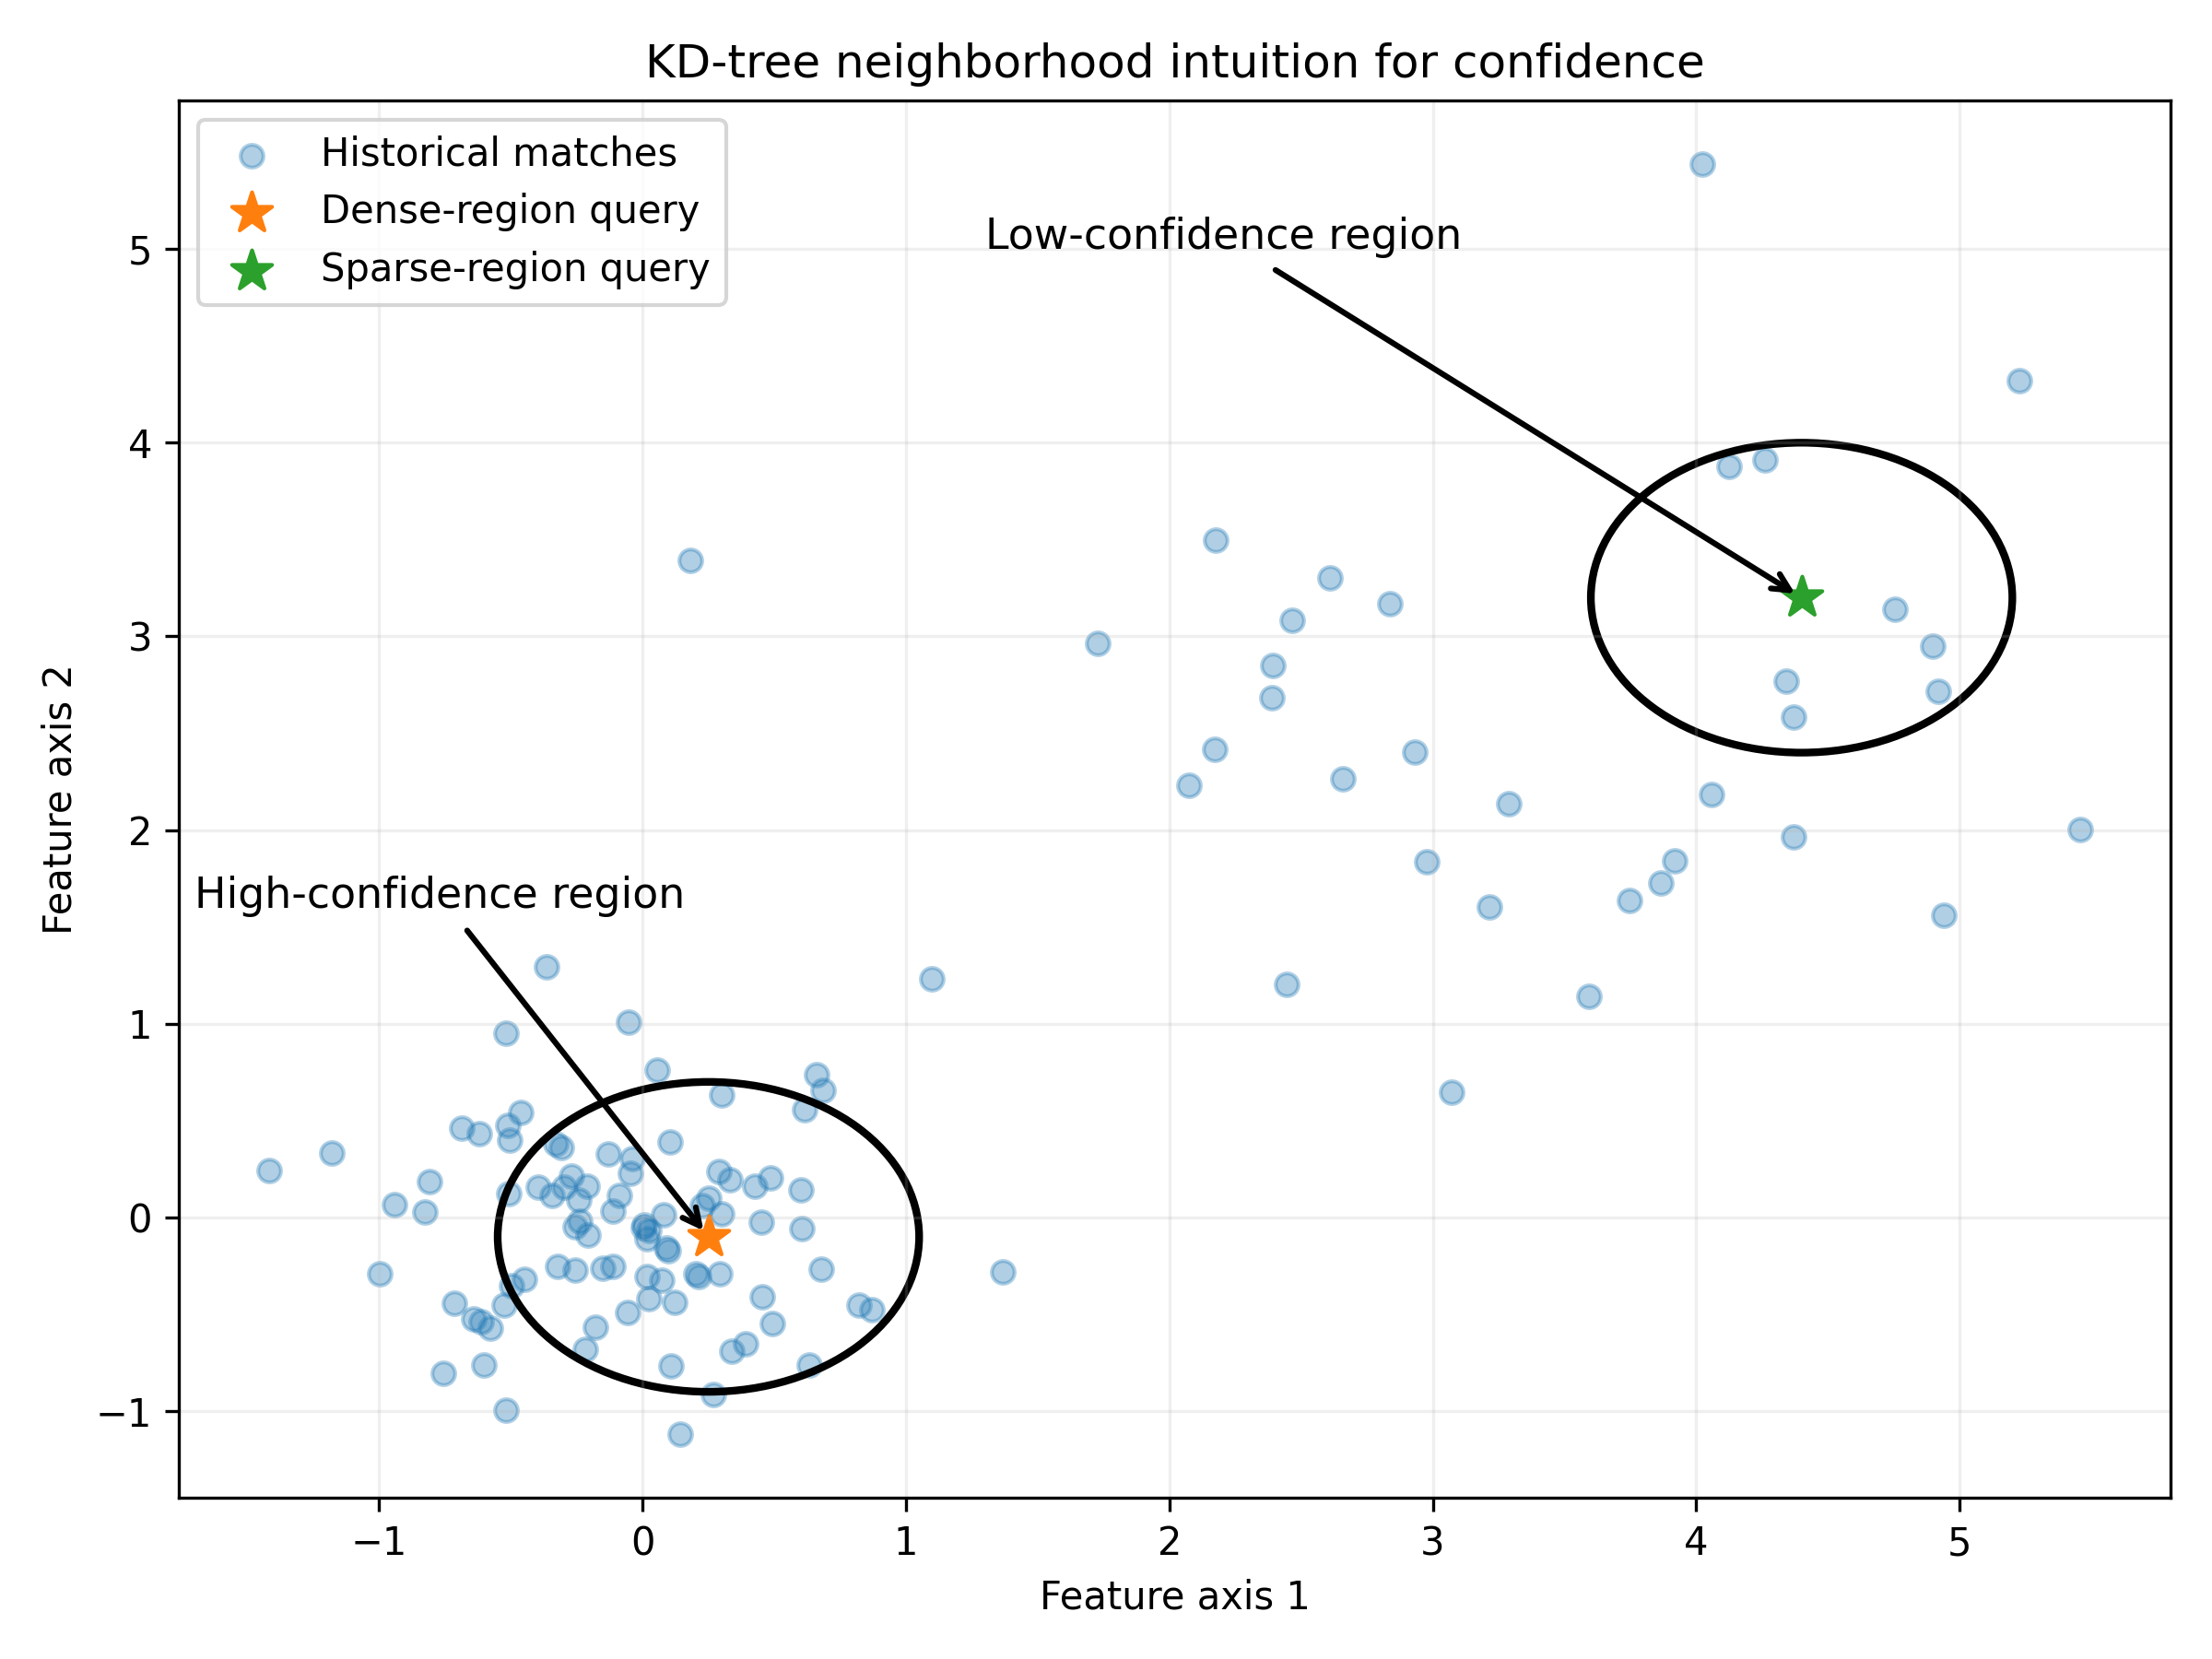
\includegraphics[width=0.80\linewidth]{poster_images/kdtree_diagram.png}
            \end{center}
            \vspace*{0.20cm}
        }

        % extra separation so the final output box does not visually merge upward
        \vspace*{0.20cm}

        \posterboxthree{Model Prediction Output}{
            \vspace*{0.22cm}
            \begin{center}
                % IMAGE: poster_images/sample_prediction.png
                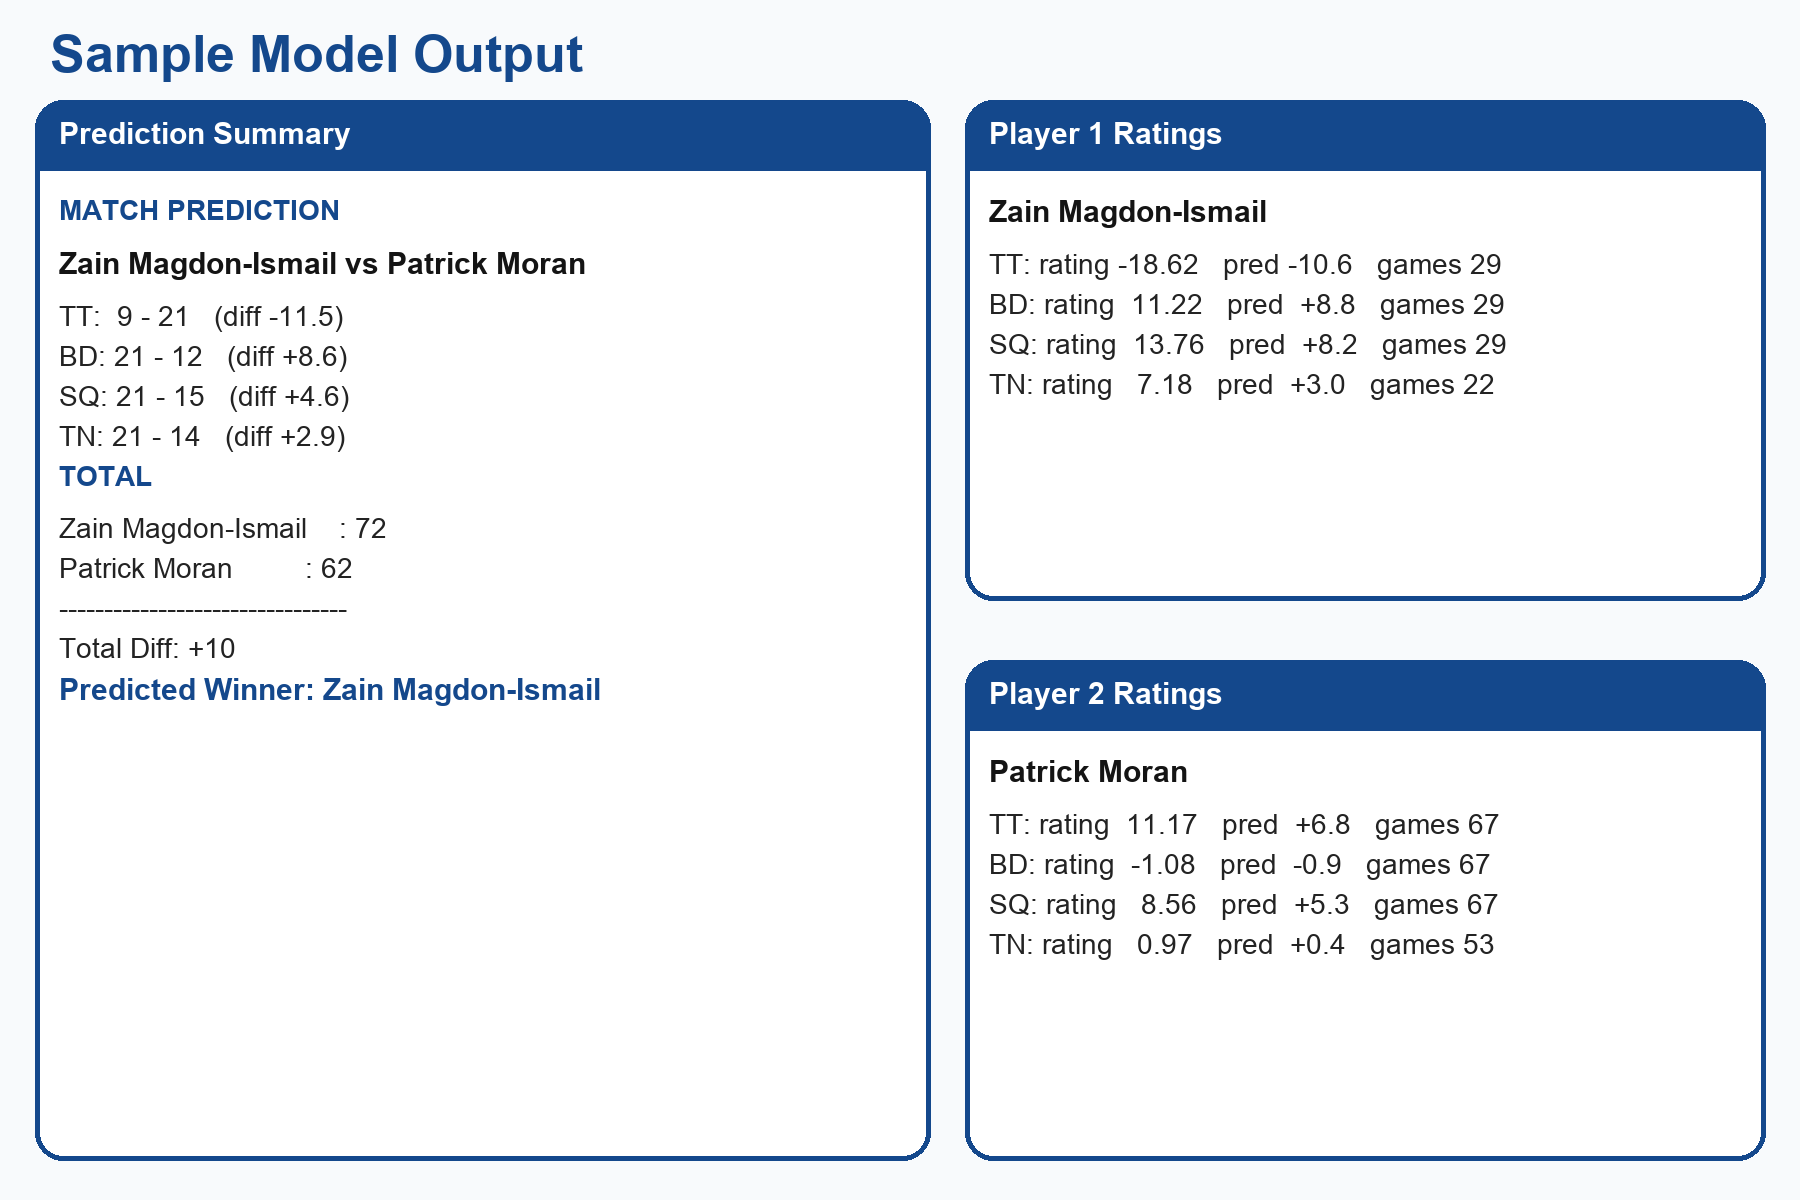
\includegraphics[width=0.9\linewidth]{poster_images/sample_prediction.png}
            \end{center}
            \vspace*{0.20cm}
        }

    \end{minipage}

\end{minipage}

\end{document}